% \documentclass[border={10pt 10pt 80pt 10pt},tikz,multi]{standalone}
\documentclass[border={10pt 10pt 10pt 10pt},tikz,multi]{standalone}
\usetikzlibrary{angles,shadows.blur,positioning,backgrounds}
\usepackage[dvipsnames]{xcolor}
\usepackage{amsmath}
\usepackage{amssymb}

% Define alias for minimum width and height
\newcommand{\globalminwidth}{15cm}
\newcommand{\globalminheight}{12cm}

\newcommand{\scopeminwidth}{(\globalminwidth - 1cm) / 2 - 0.5cm}
\newcommand{\scopeminheight}{\globalminheight / 3}


\begin{document}
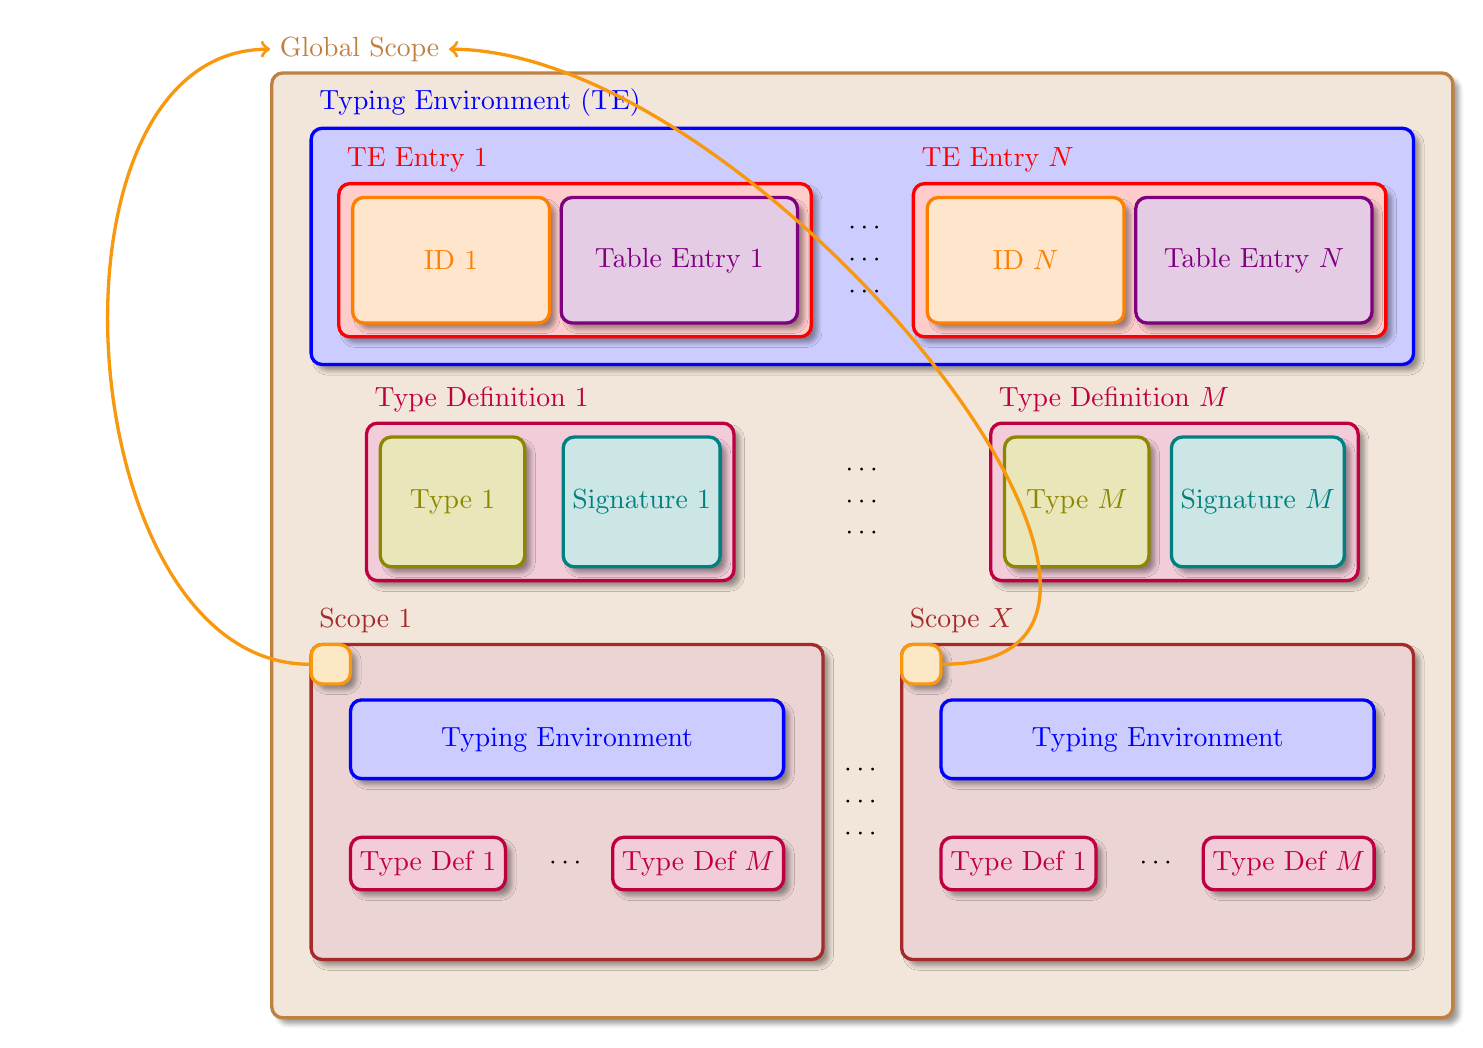
\begin{tikzpicture}

    % FIRST TRY
    % \node[draw, very thick, rounded corners, fill=Black!10, blur shadow={shadow blur steps=5}, minimum width=10cm, minimum height=6cm] (LV) {};
    % \node[] (LV_label) [above right=0cm and 0cm of LV.north west] {Language Variant};

    % SECOND TRY
    % \node[draw, rectangle, very thick, rounded corners, fill=Black!10, blur shadow={shadow blur steps=5}, minimum width=10cm, minimum height=6cm, label={[above left=0pt]Language Variant}] (LV) {};

    % THIRD TRY
    \node[draw=brown,
          rectangle,
          very thick,
          rounded corners,
          fill=brown!20,
          blur shadow={shadow blur steps=5},
          minimum width=\globalminwidth,
          minimum height=\globalminheight] (GS) at (0,0) {};
    \node[text=brown, above right] (GST) at (GS.north west) {Global Scope};

    % ====================================================================
    \node[draw=blue,
          text=blue,
          rectangle,
          very thick,
          rounded corners,
          fill=blue!20,
          blur shadow={shadow blur steps=5},
          minimum width=\globalminwidth - 1cm,
          minimum height=\globalminheight / 4,
          below=20pt] (TE) at (GS.north) {};
    \node[text=blue, above right]  at (TE.north west) {Typing Environment (TE)};

    \node[draw=red,
          text=red,
          rectangle,
          very thick,
          rounded corners,
          fill=red!20,
          blur shadow={shadow blur steps=5},
          minimum width=(\globalminwidth - 1cm) / 2 - 1cm,
          minimum height=(\globalminheight / 4) - 30pt,
          below right=20pt and 10pt] (TE1) at (TE.north west) {};
    \node[text=red, above right] at (TE1.north west) {TE Entry $1$};

    \node[draw=orange,
          text=orange,
          rectangle,
          very thick,
          rounded corners,
          fill=orange!20,
          blur shadow={shadow blur steps=5},
          minimum width=((\globalminwidth - 1cm) / 2 - 1cm) / 2 - 0.5cm,
          minimum height=((\globalminheight / 4) - 30pt) - 10pt,
          below right=5pt and 5pt] (TEID1) at (TE1.north west) {ID $1$};
    \node[draw=violet,
          text=violet,
          rectangle,
          very thick,
          rounded corners,
          fill=violet!20,
          blur shadow={shadow blur steps=5},
          minimum width=((\globalminwidth - 1cm) / 2 - 1cm) / 2,
          minimum height=((\globalminheight / 4) - 30pt) - 10pt,
          below left=5pt and 5pt] (TEE2) at (TE1.north east) {Table Entry $1$};


    % dots
    \node[right=0.325cm] (Dots1) at (TE1.east) {$\cdots$};
    \node[above] (Dots2) at (Dots1.north) {$\cdots$};
    \node[below] (Dots3) at (Dots1.south) {$\cdots$};

    \node[draw=red,
          text=red,
          rectangle,
          very thick,
          rounded corners,
          fill=red!20,
          blur shadow={shadow blur steps=5},
          minimum width=(\globalminwidth - 1cm) / 2 - 1cm,
          minimum height=(\globalminheight / 4) - 30pt,
          below left=20pt and 10pt] (TEN) at (TE.north east) {};
    \node[text=red, above right] at (TEN.north west) {TE Entry $N$};

    \node[draw=orange,
          text=orange,
          rectangle,
          very thick,
          rounded corners,
          fill=orange!20,
          blur shadow={shadow blur steps=5},
          minimum width=((\globalminwidth - 1cm) / 2 - 1cm) / 2 - 0.5cm,
          minimum height=((\globalminheight / 4) - 30pt) - 10pt,
          below right=5pt and 5pt] (TEIDN) at (TEN.north west) {ID $N$};

    \node[draw=violet,
          text=violet,
          rectangle,
          very thick,
          rounded corners,
          fill=violet!20,
          blur shadow={shadow blur steps=5},
          minimum width=((\globalminwidth - 1cm) / 2 - 1cm) / 2,
          minimum height=((\globalminheight / 4) - 30pt) - 10pt,
          below left=5pt and 5pt] (TEEN) at (TEN.north east) {Table Entry $N$};

    % ====================================================================
    \node[draw=purple,
          text=purple,
          rectangle,
          very thick,
          rounded corners,
          fill=purple!20,
          blur shadow={shadow blur steps=5},
          minimum width=(\globalminwidth - 1cm) / 3,
          minimum height=\globalminheight / 6,
          below right=20pt and 20pt] (TS1) at (TE.south west) {};
    \node[text=purple, above right] at (TS1.north west) {Type Definition $1$};

    \node[draw=olive,
          text=olive,
          rectangle,
          very thick,
          rounded corners,
          fill=olive!20,
          blur shadow={shadow blur steps=5},
          minimum width=(((\globalminwidth - 1cm) / 3) / 2) - 0.5cm,
          minimum height=(\globalminheight / 6) - 10pt,
          below right=5pt and 5pt] (TY1) at (TS1.north west) {Type $1$};

     \node[draw=teal,
          text=teal,
          rectangle,
          very thick,
          rounded corners,
          fill=teal!20,
          blur shadow={shadow blur steps=5},
          minimum width=(((\globalminwidth - 1cm) / 3) / 2) - 0.5cm,
          minimum height=(\globalminheight / 6) - 10pt,
          below left=5pt and 5pt] (SGN1) at (TS1.north east) {Signature $1$};


    % dots
    \node[right=(\globalminwidth - 1cm) / 11] (Dots1) at (TS1.east) {$\cdots$};
    \node[above] (Dots2) at (Dots1.north) {$\cdots$};
    \node[below] (Dots3) at (Dots1.south) {$\cdots$};

    \node[draw=purple,
          text=purple,
          rectangle,
          very thick,
          rounded corners,
          fill=purple!20,
          blur shadow={shadow blur steps=5},
          minimum width=(\globalminwidth - 1cm) / 3,
          minimum height=\globalminheight / 6,
          below left=20pt and 20pt] (TS2) at (TE.south east) {};
    \node[text=purple, above right] at (TS2.north west) {Type Definition $M$};

    \node[draw=olive,
          text=olive,
          rectangle,
          very thick,
          rounded corners,
          fill=olive!20,
          blur shadow={shadow blur steps=5},
          minimum width=(((\globalminwidth - 1cm) / 3) / 2) - 0.5cm,
          minimum height=(\globalminheight / 6) - 10pt,
          below right=5pt and 5pt] (TY2) at (TS2.north west) {Type $M$};

    \node[draw=teal,
          text=teal,
          rectangle,
          very thick,
          rounded corners,
          fill=teal!20,
          blur shadow={shadow blur steps=5},
          minimum width=(((\globalminwidth - 1cm) / 3) / 2) - 0.5cm,
          minimum height=(\globalminheight / 6) - 10pt,
          below left=5pt and 5pt] (SGN2) at (TS2.north east) {Signature $M$};

    % ====================================================================

    \node[draw=Brown,
          text=Brown,
          rectangle,
          very thick,
          rounded corners,
          fill=Brown!20,
          blur shadow={shadow blur steps=5},
          minimum width=\scopeminwidth,
          minimum height=\scopeminheight,
          below right=100pt and 0pt] (S1) at (TE.south west) {};
    \node[text=Brown, above right] at (S1.north west) {Scope $1$};




    \node[right=0.125cm] (Dots1) at (S1.east) {$\cdots$};
    \node[above] (Dots2) at (Dots1.north) {$\cdots$};
    \node[below] (Dots3) at (Dots1.south) {$\cdots$};

    \node[draw=Brown,
          text=Brown,
          rectangle,
          very thick,
          rounded corners,
          fill=Brown!20,
          blur shadow={shadow blur steps=5},
          minimum width=\scopeminwidth,
          minimum height=\scopeminheight,
          below left=100pt and 0pt] (SX) at (TE.south east) {};
    \node[text=Brown, above right] at (SX.north west) {Scope $X$};



    % ====================================================================

    \node[draw=YellowOrange,
          text=YellowOrange,
          rectangle,
          very thick,
          rounded corners,
          fill=YellowOrange!20,
          blur shadow={shadow blur steps=5},
          minimum width=0.5cm,
          minimum height=0.5cm,
          below right = 0pt and 0pt] (P1) at (S1.north west) {};
    % Arrow from P1 to GST
    \draw[YellowOrange, ->, very thick] (P1) to[out=180, in=180] (GST.west);


    \node[draw=blue,
          text=blue,
          rectangle,
          very thick,
          rounded corners,
          fill=blue!20,
          blur shadow={shadow blur steps=5},
          minimum width=\scopeminwidth - 1cm,
          minimum height=\scopeminheight / 4,
          below=20pt] (TE) at (S1.north) {Typing Environment};


    % ====================================================================
    \node[draw=purple,
          text=purple,
          rectangle,
          very thick,
          rounded corners,
          fill=purple!20,
          blur shadow={shadow blur steps=5},
          minimum width=(\scopeminwidth - 1cm) / 3,
          minimum height=\scopeminheight / 6,
          below right=20pt and 0pt] (TS1) at (TE.south west) {Type Def $1$};

    % dots
    \node[right=(\scopeminwidth - 2cm) / 11] (Dots1) at (TS1.east) {$\cdots$};

    \node[draw=purple,
          text=purple,
          rectangle,
          very thick,
          rounded corners,
          fill=purple!20,
          blur shadow={shadow blur steps=5},
          minimum width=(\scopeminwidth - 1cm) / 3,
          minimum height=\scopeminheight / 6,
          below left=20pt and 0pt] (TS2) at (TE.south east) {Type Def $M$};

    % ====================================================================

    % ====================================================================

    \node[draw=YellowOrange,
          text=YellowOrange,
          rectangle,
          very thick,
          rounded corners,
          fill=YellowOrange!20,
          blur shadow={shadow blur steps=5},
          minimum width=0.5cm,
          minimum height=0.5cm,
          below right = 0pt and 0pt] (P1) at (SX.north west) {};
    % Arrow from P1 to GST
    \draw[YellowOrange, ->, very thick] (P1) to[out=0, in=0] (GST.east);

    \node[draw=blue,
          text=blue,
          rectangle,
          very thick,
          rounded corners,
          fill=blue!20,
          blur shadow={shadow blur steps=5},
          minimum width=\scopeminwidth - 1cm,
          minimum height=\scopeminheight / 4,
          below=20pt] (TE) at (SX.north) {Typing Environment};


    % ====================================================================
    \node[draw=purple,
          text=purple,
          rectangle,
          very thick,
          rounded corners,
          fill=purple!20,
          blur shadow={shadow blur steps=5},
          minimum width=(\scopeminwidth - 1cm) / 3,
          minimum height=\scopeminheight / 6,
          below right=20pt and 0pt] (TS1) at (TE.south west) {Type Def $1$};

    % dots
    \node[right=(\scopeminwidth - 2cm) / 11] (Dots1) at (TS1.east) {$\cdots$};

    \node[draw=purple,
          text=purple,
          rectangle,
          very thick,
          rounded corners,
          fill=purple!20,
          blur shadow={shadow blur steps=5},
          minimum width=(\scopeminwidth - 1cm) / 3,
          minimum height=\scopeminheight / 6,
          below left=20pt and 0pt] (TS2) at (TE.south east) {Type Def $M$};

\end{tikzpicture}

\end{document}


